\documentclass[dvipdfmx]{jarticle}
\pagestyle{empty}
\usepackage{tikz}
\usetikzlibrary{shapes,calc,automata}
\begin{document}
\begin{tabular}{ccccc}
 & $\mathsf{NDec}(\mathsf{NDec}|\mathsf{Dec})^\ast$ & \qquad &
 & $\mathsf{NZDec}\,\mathsf{Dec}^\ast$\\
  $A_{id}$: & & & $A_{cnst}$: &\\[-10pt]
 & 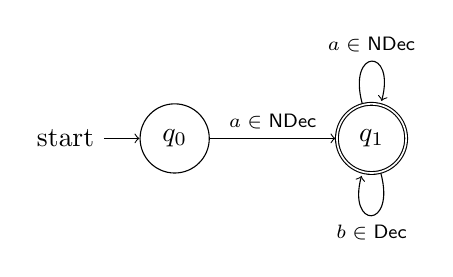
\begin{tikzpicture}[node distance=2.5cm,auto]
\node[state,initial] (q0) {$q_0$};
\node[state,accepting] (q1) [right of=q0] {$q_1$};
\path[->] (q0) edge node {\scriptsize $a\in\mathsf{NDec}$} (q1);
\path[->] (q1) edge [loop above] node {\scriptsize $a\in\mathsf{NDec}$} ();
\path[->] (q1) edge [loop below] node {\scriptsize $b\in\mathsf{Dec}$} ();
\end{tikzpicture} & & &
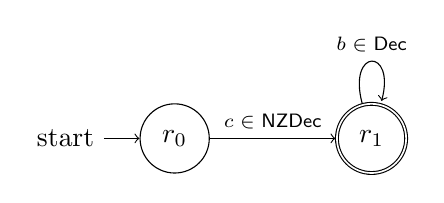
\begin{tikzpicture}[node distance=2.5cm,auto]
  \node[state,initial] (r0) {$r_0$};
  \node[state,accepting] (r1) [right of=r0] {$r_1$};
  \path[->] (r0) edge node {\scriptsize $c\in\mathsf{NZDec}$} (r1);
  \path[->] (r1) edge [loop above] node {\scriptsize $b\in\mathsf{Dec}$} ();
\end{tikzpicture}\\
\multicolumn{2}{c}{(a)識別子トークンを受理するオートマトン} & & 
\multicolumn{2}{c}{(b)自然数定数トークンを受理するオートマトン}
\\[10pt]
\multicolumn{5}{l}{$A_{id}\cup A_{cnst}$:}\\
& \multicolumn{4}{c}{
  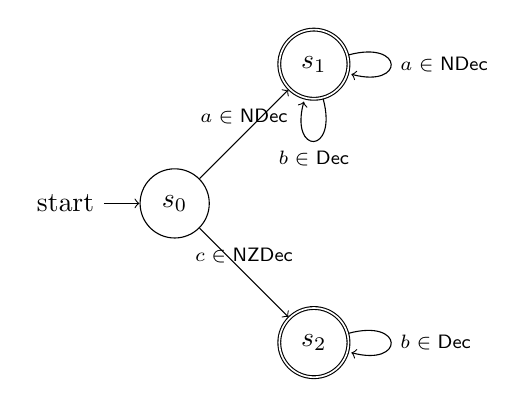
\begin{tikzpicture}[node distance=2.5cm,auto]
    \node[state,initial] (s0) {$s_0$};
    \node[state,accepting] (s1) [above right of=s0] {$s_1$};
    \node[state,accepting] (s2) [below right of=s0] {$s_2$};
    \path[->] (s0) edge [above] node {\scriptsize $a\in\mathsf{NDec}$} (s1);
    \path[->] (s1) edge [loop right] node {\scriptsize $a\in\mathsf{NDec}$} ();
    \path[->] (s1) edge [loop below] node {\scriptsize $b\in\mathsf{Dec}$} ();
    \path[->] (s0) edge [above] node {\scriptsize $c\in\mathsf{NZDec}$} (s2);
    \path[->] (s2) edge [loop right] node {\scriptsize $b\in\mathsf{Dec}$} ();
  \end{tikzpicture}
}\\
\multicolumn{5}{c}{(c)両方のトークンを受理するオートマトン}
\end{tabular}
\end{document}